\chapter{Výsledky práce a možnosti rozšírenia}
\section{RGB kamera vs hĺbkový senzor}
Jedným z hlavných cieľov tejto práce je porovnať využitie 3D a 2D technológie pri sledovaní prechodov osôb cez virtuálnu bránu. Za týmto účelom boli vytvorené dva programy, ktoré sa podrobili dôkladným testom, ktorých výsledky boli následne porovnané. 

\subsection{Testovanie v reálnom prostredí farmaceutickej firmy}
Za účelom testovania aplikácie boli vytvorené dva 3 - 4 hodinové záznamy zo špedičnej prevádzky farmaceutickej firmy. Zariadenie bolo umiestnené na miesto frekventovaného prechodu, ktorý predstavoval spojovacie dvere medzi dvoma oddeleniami. Zamestnanci prechádzali osobitne, ale aj v skupinách a väčšina v rukách alebo na ručnom vozíku prenášala tovar, ktorý predstavoval kopy krabíc naukladaných na sebe. 

Obe kamery boli umiestnené podľa konceptu (kapitola \ref{sec:draft}) tak, aby snímali približne rovnaký bod prechodu. Jednotlivé programy uspeli nasledovne:  

\begin{figure}[H]
  \centering
  \begin{minipage}[b]{0.43\textwidth}
    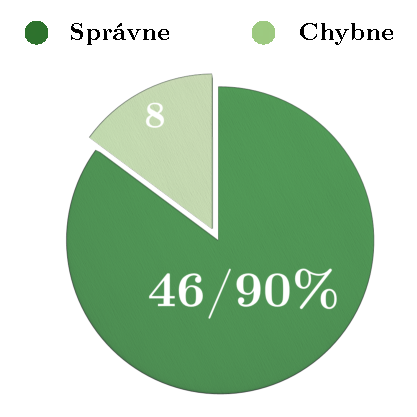
\includegraphics[width=\textwidth]{images/2D_graph_medart}
    \caption{2D úspešnosť detekcie.}
  \end{minipage}
  \hfill
  \begin{minipage}[b]{0.43\textwidth}
    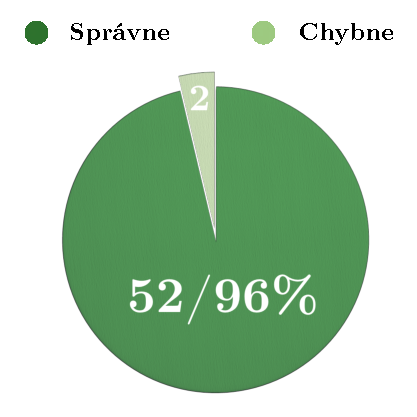
\includegraphics[width=\textwidth]{images/3D_graph_medart}
    \caption{3D úspešnosť detekcie.}
  \end{minipage}
\end{figure}

Všetky chyby spôsobené v programe používajúci \textbf{2D snímanie scény} boli spôsobené vozíkom, ktorý človek ťahal za sebou ako je znázornené na obrázku. 

\begin{figure}[H]
  \centering
  \begin{minipage}[b]{0.48\textwidth}
    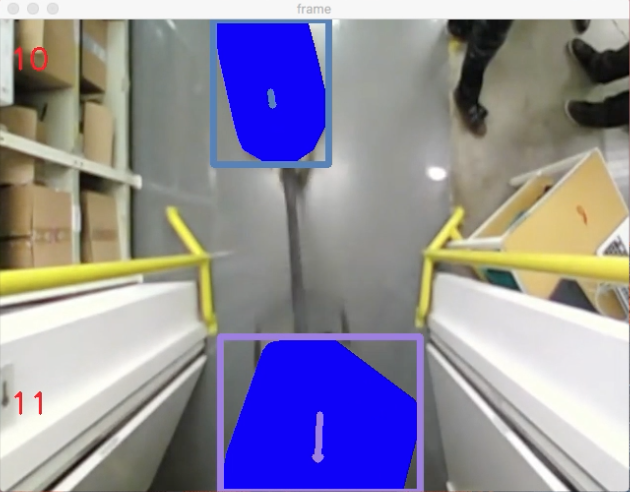
\includegraphics[width=\textwidth]{images/handCard}
    \caption{Segmentácia snímku programom.}
  \end{minipage}
  \hfill
  \begin{minipage}[b]{0.48\textwidth}
    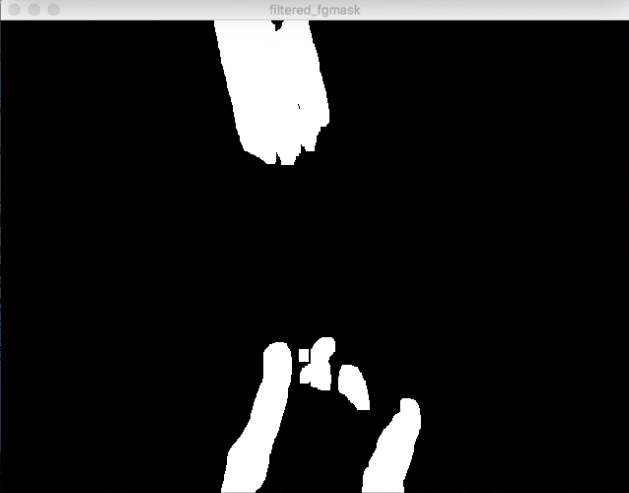
\includegraphics[width=\textwidth]{images/handCard_fmask}
    \caption{Binárna maska zo substractora.}
  \end{minipage}
\end{figure}  

Na vyriešenie opísanej chyby je nutné disponovať väčším množstvom informácií z obrazu. S použitou technológiou nie je možné spoľahlivo rozoznať, či sa jedná o vozík, ktorý je ťahaný za človekom alebo o ďalšieho človeka kráčajúceho za ním. V prípade, že zamestnanec vozík tlačil pred sebou, program dokázal jednotlivé kontúry pospájať do jednej veľkej a tak človek aj vozík predstavovali jeden objekt. Ďalším zdrojom chýb bol extrémne naplnený vozík, ktorého náklad bol tak vysoký, že pri prechode zabral celý obraz snímaný kamerou. Tento prípad sa programu nepodarilo detekovať a odstrániť.

V rovnakých podmienkach si program, ktorý používa \textbf{3D metódu snímania} poradil o niečo lepšie. Na 54 veľmi náročných prechodoch, situáciu vyhodnotil zle len 2x. Obe chyby boli spôsobené už spomínaným vozíkom s veľmi vysoko naloženým nákladom. Avšak ten istý vozík prechádzal štyrikrát, čiže v polovici prípadov si program využívajúci 3D poradil aj s touto hraničnou situáciou na rozdiel od programu využívajúceho 2D snímanie, ktorý zlyhal vo všetkých štyroch prípadoch. 

\begin{figure}[H]
  \centering
  \begin{minipage}[b]{0.48\textwidth}
    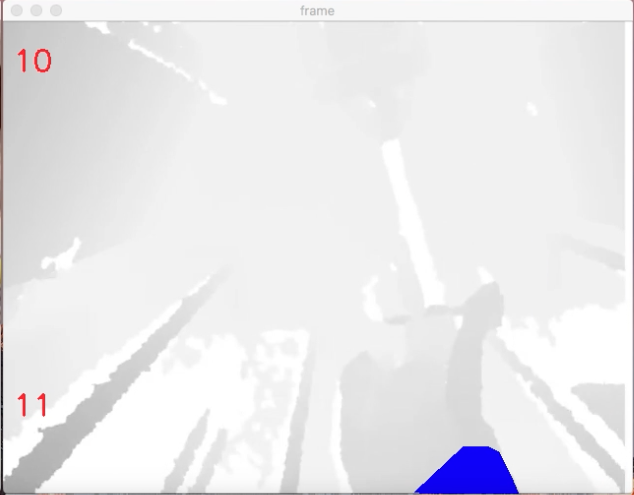
\includegraphics[width=\textwidth]{images/handCard_3D}
    \caption{Segmentácia snímku 3D programom v rovnakej situácií ako obrázok 5.3.}
  \end{minipage}
  \hfill
  \begin{minipage}[b]{0.48\textwidth}
    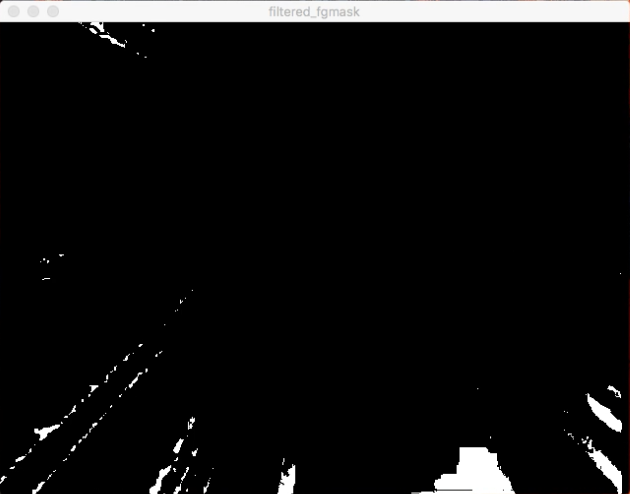
\includegraphics[width=\textwidth]{images/handCard_fmask_3D}
    \caption{Binárna maska zo substractora  v rovnakej situácií ako obrázok 5.4.}
  \end{minipage}
\end{figure}  

\subsection{Dlhodobé testovanie v simulovaných podmienkach}
V priebehu vývoja oboch algoritmov, vzniklo veľké množstvo videí, na ktorých boli simulované rôzne situácie, ktoré v dynamickom prostredí virtuálnej brány môžu nastať. Ako napríklad prechod jednej, dvoch alebo viacerých osôb jedným alebo opačným smerom, zrazenie sa dvoch a viacerých ľudí, "motanie sa" v priestoroch virtuálnej brány, prebehnutie, skákanie a iné situácie. S využitím všetkých záznamov bola vypočítaná úspešnosť oboch algoritmov na vzorke stoviek prechodov.    

\begin{itemize}
\item Program, ktorý na snímanie využíva \textbf{2D snímanie priestoru} dosiahol úspešnosť na hranici \textbf{94\%}
\item Program, ktorý na snímanie využíva \textbf{3D snímanie priestoru} dosiahol úspešnosť \textbf{98\%}
\end{itemize}

Hlavným dôvodom výraznejšieho úspechu 3D technológie je stabilnejšie určenie primárneho bodu v kontúre (hlava). Vďaka tomu, predikčný algoritmus pracoval s presnejšími hodnotami a v prípade náhlej straty kontúry objektu, dokázal s veľkou úspešnosťou opätovne kontúru nájsť na základe predikcie nasledujúceho pohybu. Pri 2D technológií obrazu je veľmi náročné určiť stabilný bod. Preto sa algoritmus opiera o hodnotu ťažiska jednotlivých kontúr. Tvar a veľkosť kontúry je však veľmi menná, čo spôsobuje, že aj poloha ťažiska nemá lineárny priebeh (vysoký šum). Ďalšou výhodou 3D technológie, je možnosť odfiltrovať objekty, podľa ich výšky.

\vspace{5mm}


\subsection{Bezpečnostné problémy}
Porovnanie v tejto kategórií je veľmi prínosné vzhľadom na ďalšie využitie v bezpečnostných aplikáciach. Obe technológie snímania majú svoje silné a slabé stránky.

\subsubsection{3D technológia}
Prvý problém predstavuje situácia, ak je stanovený výškový prach detekcie objektov (prípad s vozíkmi) alebo hĺbkový snímač nemá dostatočne veľký dosah snímania (až po zem). V týchto prípadoch môže útočník podliezť tento prah snímania. Ďalším potenciálnym problémom je, že hĺbkové senzory nevedia vykonať meranie oproti istému druhu materiálov, ako napríklad sklo. Na druhej strane sú však mnohé výhody, ako napríklad  nezávislosť na osvetlení priestoru. Snímanie funguje aj za úplnej tmy. 

\subsubsection{2D technológia}
Slabinou tohto systému je samotný background substractor, ktorý pracuje na princípe učenia sa pozadia. To znamená, že ak sa potencionálny útočník postaví do obrazu a bude tam stáť dostatočne dlho, systém sa ho naučí ako súčasť pozadia. Takto môže postupne prejsť celý prechod. Ďalším všeobecným problémom technológie je svetlo. Prechod musí byť vždy dobre osvetlený (homogénne svetlo), inak detekcia nie je možná. 

\vspace{5mm}

\subsection{Zhodnotenie}
Systém založený na 2D snímaní pomocou kamery je vhodný pre aplikácie, kde nie je požadovaná extrémna presnosť, ale nízka cena. Príkladom môže byť obchod, ktorý si vedie štatistiku návštev. Na druhej strane 3D snímanie pomocou hĺbkomerov je vhodné pre bezpečnostné aplikácie súvisiace s objektovým zabezpečením. Výhodou je pridaný údaj o hĺbke, vysoká presnosť snímania, spoľahlivosť.       


\section{Možnosti rozšírenia}
Najvýznamnejšou možnosťou rozšírenia projektu je využitie aplikácie ako základ pre objektovú bezpečnosť. Ďalším krokom vpred, by malo byť priradenie identity jednotlivým objektom. To možno dosiahnuť rôznym spôsobom: 

\begin{itemize}
\item \textit{Vysoko-výkonového RFID} - jednalo by sa teda o identitu na základe vlastníctva (čip). Tento spôsob však prináša technologické problémy, keďže by bolo veľmi ťažké zabezpečiť, aby RFID antény príjmali signál len od čipov nachádzajúcich sa v priestore brány. 
\item \textit{Biometrické systémy} - na základe tvárovej biometrie by bolo možné priradiť identitu danému človeku. V spojení s týmto projektom by bolo možné odhaliť potencionálneho útočníka, ktorý odmietne interakciu s takýmto biometrickým zariadením (musí sa pozrieť do kamery). 
\end{itemize}


Ďalšia možnosť spočíva v dobudovaní serverovej infraštruktúry a vytvorenií informačného systému pre správu štatistík o návštevnosti nejakého miesta. Cieľovým zákazníkom takéhoto systému sú všetky obchodné reťazce, ktorých zaujíma návštevnosť svojich predajní v závislosti na čase či mieste.

































